
%%% Local Variables: 
%%% mode: latex
%%% TeX-master: t
%%% End: 


\documentclass{sig-alternate}

% Housekeeping
\usepackage{amsmath}
\usepackage{amssymb}

\usepackage{cite}
\usepackage{algorithmic}
\usepackage{array}
\usepackage{graphicx}
\graphicspath{{./}{./Figure/}}

\usepackage{url}





\begin{document}
\title{Improving Building Energy Efficiency by Kinect-based Occupancy
  Tracking and Mobility Detecting System}

\numberofauthors{1}
\author{
\alignauthor
Haleimah Al Zeyoudi\quad Yanan Xiao\quad Chi-Kin Chau\\
\affaddr{Masdar Institute of Science and Technology}
\affaddr{P.O. Box 54224}
\affaddr{Abu Dhabi, UAE}
\email{\{hzeyoudi,yxiao,ckchau\}@masdar.ac.ae}
}

% \numberofauthors{1}
% \author{
% \alignauthor
% Some author
% }


\maketitle{}



\begin{abstract}
  Nowadays, most building air conditioning systems still operate on a
  fixed schedule rather than real-time occupancy. In our study, we
  make an occupancy tracking software based on Kinect to reflect the
  number of people in a open lab. We then build a Markov Chain (MC)
  model after dividing the open area into 4 zones and calculating its
  occupancy respectively. When applying the real-time schedule of one
  week to a building model created with eQuest, we obtain a 22.1\%
  energy reduction in space cooling.
\end{abstract}

% I comment out this part. It seems that it's useless.

% \category{C.3}{Special-purpose and application-based
%   systems}{Real-time and embedded systems}

% \terms{Algorithms, Design, Management}

% \keywords{Wireless sensor networks, Markov chain, Simulation}





% What the heck am I reading.


\section{Introduction}
\label{sec:introduction}
At the core of energy consumption in modern buildings is Heating Ventilation
and Air Conditioning (HVAC) systems which are designed to operate at
full capacity most of the time because it's often assumed a maximum
occupancy. Although current HVAC systems are equipped with sensors,
their management and control systems ignore the dynamic nature 
occupancy patterns in buildings. In addition, they are unable to
proactively adjust to occupants' comfort levels. Understanding human
mobility and occupancy patterns are key factors in successfully
managing HVAC systems in buildings. The main contribution of our paper
is to propose an energy-saving model based on occupancy patterns of
human mobility in buildings. The most important features of the system
are as follows: a) A real-time detection and tracking of human
mobility in buildings based on Kinect. b) An occupancy prediction
mechanism based on MC. 
% This part should be concised.
\par






\section{Implementation}
\label{sec:implementation}

\subsection{Kinect-based Occupancy Counting Software}
Our Occupancy Counting software is written using Microsoft Visual
C\# 2010, project WPF application programmed using C\#
and XML languages. Both types of Kinect are used and tested to insure
that it works properly, i.e. Xbox Kinect and Kinect for Windows. The
software, should be run on windows 7 or above, after installing Kinect
sensor driver successfully.  

\begin{enumerate}
  \item \textbf{Kinect initialization start:} This function will look up for any connected Kinect devices to your computer.  If no device is connected: a box message will appear to inform you about this fact.  The software display both RGB and Depth image,  Figure \ref{fig:guioverview} show the GUI of our software.

     \begin{figure}[!ht]
  \begin{center}
	  	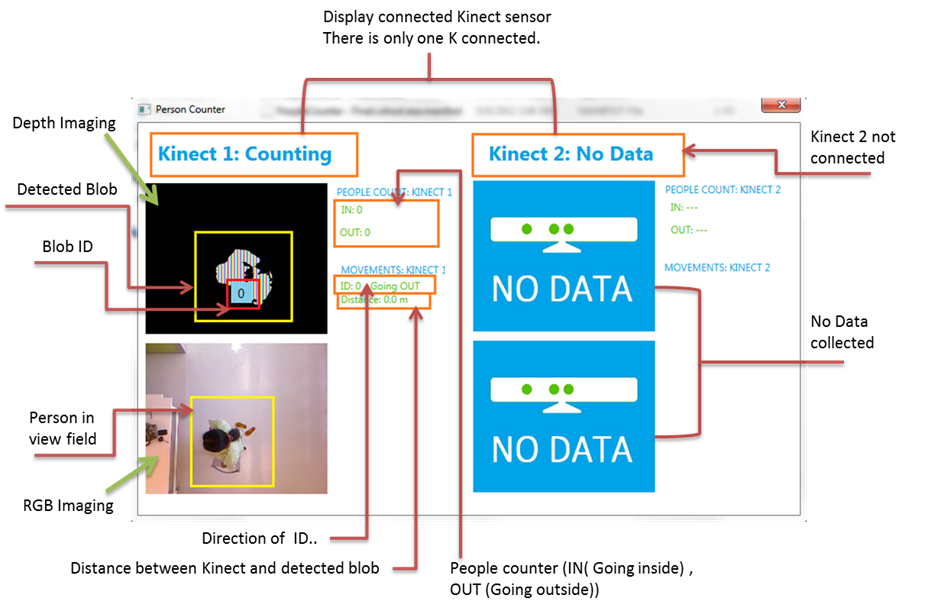
\includegraphics[width=1.1\columnwidth]{swm.png}
  \end{center}
  \caption{Overview of the GUI of our Kinect-based Occupancy Counter x.}
  \label{fig:guioverview}
\end{figure}
\item \textbf{Capture frame events}: As part of the initialization,  it makes sure that both RGB and Depth imaging are captured.
ColorImageFrameReadyEventArgs:	The event arguments provided in a KinectSensor. ColorFrameReady event when a frame of color data is ready.
\item \textbf{Depth camera feed generator:} Contains a per-frame buffer for depth data streamed out of a sensor.  Also provides access to the dimensions and format of the data in addition to mapping between skeleton and color coordinate spaces.  Once our Depth imaging is ready, we can start tracking blobs and draw markers.
\item \textbf{Generate Markers :} This draws a rectangle blue box  with unique ID of people that is used is temporarily  for the detection of multiple subjects passing in the field view.

\end{enumerate}


\begin{figure} [!ht]
  \begin{center}
	  	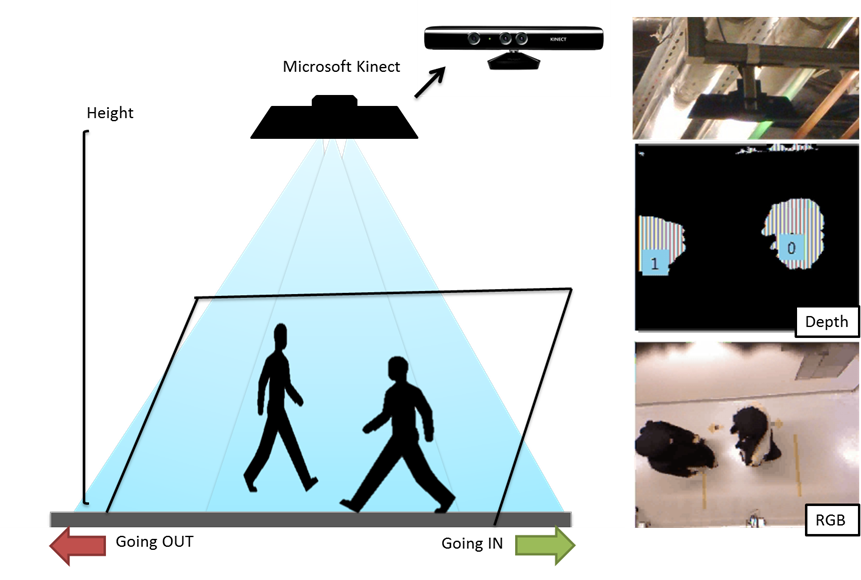
\includegraphics[width=1.05\columnwidth]{minisys.png}
  \end{center}
  \caption{The architecture of our tracking system}\label{fig:minisys}
\end{figure}

People tracking through the Kinect sensor can be done using two methods:people tracking via human posture and an existing skeletal tracking by MSDN library. Both methods are implemented into our software to help us draw a fair comparison.

\begin{figure}[!ht]
  \centering
 	  	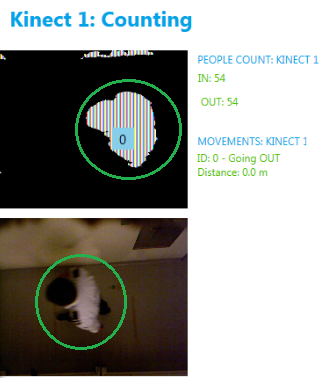
\includegraphics[width=0.7\columnwidth]{darkview.png}
  \caption{Kinect sense even in dark view, which provide a high accuracy of data capturing}
\end{figure}






\section{Results}
\label{sec:results}





% \section{Related Works}
% \label{sec:related-works}




\section{Conclusion and Future Work}
\label{sec:concl-future-work}










\bibliographystyle{plain}
\bibliography{sigproc}


\end{document}


% End of the day
% Successfully ``manage energy'' in buildings. What the heck.